\chapter{Zastosowania}
\label{cha:zastosowania}

\section{Choroby serca i pierwsza pomoc przy zawale}

Obecne społeczeństwo najwięcej kłopotów zdrowotnych ma z układem krążenia. Choroby serca są najbardziej rozpowszechnione na świecie, zwłaszcza w krajach wysoko rozwiniętych. Dlatego niezmiernie ważne jest nie tylko leczenie, ale także i zapobieganie chorobom i rehabilitacja po zawale.
\subsection{Telefony komórkowe a pierwsza pomoc}

W przypadku zawału serca niezbędna jest szybka reakcja. Często jednak stres uniemożliwia poprawne udzielenie pierwszej pomocy. Z pomocą przychodzą nam coraz szerzej dostępne inteligentne telefony komórkowe - smartphone'y. W czasopiśmie "Interventional Cardiology" (\cite{ICHoneyman2014Mobilehealthapplicationsincardiaccare}) opisane jest, w jaki sposób aplikacja mobilna może pomóc w przeprowadzeniu akcji rehabilitacyjnej:
\begin{figure}[ht!]
  \centering
    \reflectbox{%
      \includegraphics[width=0.5\textwidth]{images/cpr}}
  \caption{Schemat akcji resuscytacyjnej przy pomocy smartphone'a}
\end{figure}

\subsection{Pomoc po zawale}

Po zawale serca bardzo ważna jest praca nad stanem układu krążenia. Często jednak odległość do najbliższego szpitala jest czynnikiem zaporowym, uniemożliwiającym poprawne zadbanie o zdrowie. Ostatnie badania pokazują jednak \cite{FMottl2014Smartphoneappprovesvaluableforcardiacpatients}, iż telefon komórkowy może znacznie poprawić sytuację pacjentów pozawałowych. Aplikacja przypomina o regularnych ćwiczeniach i pozwala monitorować aktualny stan zdrowia.
\section{Monitorowanie pacjenta chorego na cukrzycę}
\label{sec:cukrzyca}

Problem cukrzycy jest również jednym z najpoważniejszych zadań, z jakimi spotyka się dzisiejsza medycyna. Dotyczy on bowiem znacznej części społeczeństwa. W artykule \cite{CDTran2012Smartphone-BasedGlucoseMonitorsandApplicationsintheManagementofDiabetes:AnOverviewof10SalientAppsandaNovelSmartphone-ConnectedBloodGlucoseMonitorUnitedStates--USGlucoseSmartphonesCellulartelephonesDiabetes} możemy znaleźć informacje na temat dostępnych na rynku aplikacji do monitorowania poziomu cukru we krwi.
\subsection{Przegląd aplikacji}
Na rynku dostępnych jest wiele aplikacji na wszystkie popularne obecnie platformy, takie jak Android, iOS czy BlackBerry OS.
\paragraph{Glucose Buddy}\mbox{}\\
Aplikacja firmy SkyHealth integruje funkcjonalność smartphone'a z danymi dostępnymi w internecie. Użytkownik może śledzić nie tylko swój poziom cukru we krwi, ale także na przykład ilość przyjmowanych składników spożywczych. Aplikacja jest darmowa.
\paragraph{Diabetes Buddy}\mbox{}\\
Płatną, ale bardziej rozwiniętą aplikacją, jest Diabetes Buddy. Umożliwia ona także monitorowanie poziomu ciśnienia krwi.
\paragraph{Log Frog}\mbox{}\\
Jedną z ciekawszych propozycji na rynku jest aplikacja Log Frog. Oferuje ona opisane wcześniej funkcjonalności, różni się jednak bardzo przyjaznym i prostym interfejsem, odpowiednim dla dzieci bądź osób starszych.

\section{Aplikacja mobilna a choroby psychiczne}
Okazuje się, iż telefony komórkowe obecnie mogą pomóc nie tylko osobom chorym z powodu dysfunkcji narządów. Także pacjenci mentalnie chorzy mogą liczyć na pomoc dzisiejszej technologii. Za pomocą odpowiednich systemów monitorowane są ich zachowania w konkretnych sytuacjach, przez co osobom opiekującym się nimi łatwiej jest dostrzec nieprawidłowości.\\
Do tej pory prowadzone badania obejmowały m. in. schizofrenię i psychozę oraz chorobę dwubiegunową \cite{IJOMHSPawelProciow2012Mobilepsychiatry:towardsimprovingthecareforbipolardisorderScience&TechnologyLifeSciences&BiomedicinePsychiatryPSYCHIATRYSSCIAMBULATORYASSESSMENTCIRCADIAN-RHYTHMSMENTAL-DISORDERSDAILY-LIFEPSYCHOLOGYCREATIVITYMOVEMENTBURDENSLEEP}. W artykule \cite{JoPNHSElias2014MobileAppsforPsychiatricNursesPsychiatric-mentalhealthnursingSmartphonesHandheldcomputersSoftware} omówione zostały aplikacje przydatne specjalistom w dziedzinie psychologii. \\ \\ \\
\begin{figure}[ht!]
  \centering
    \reflectbox{%
      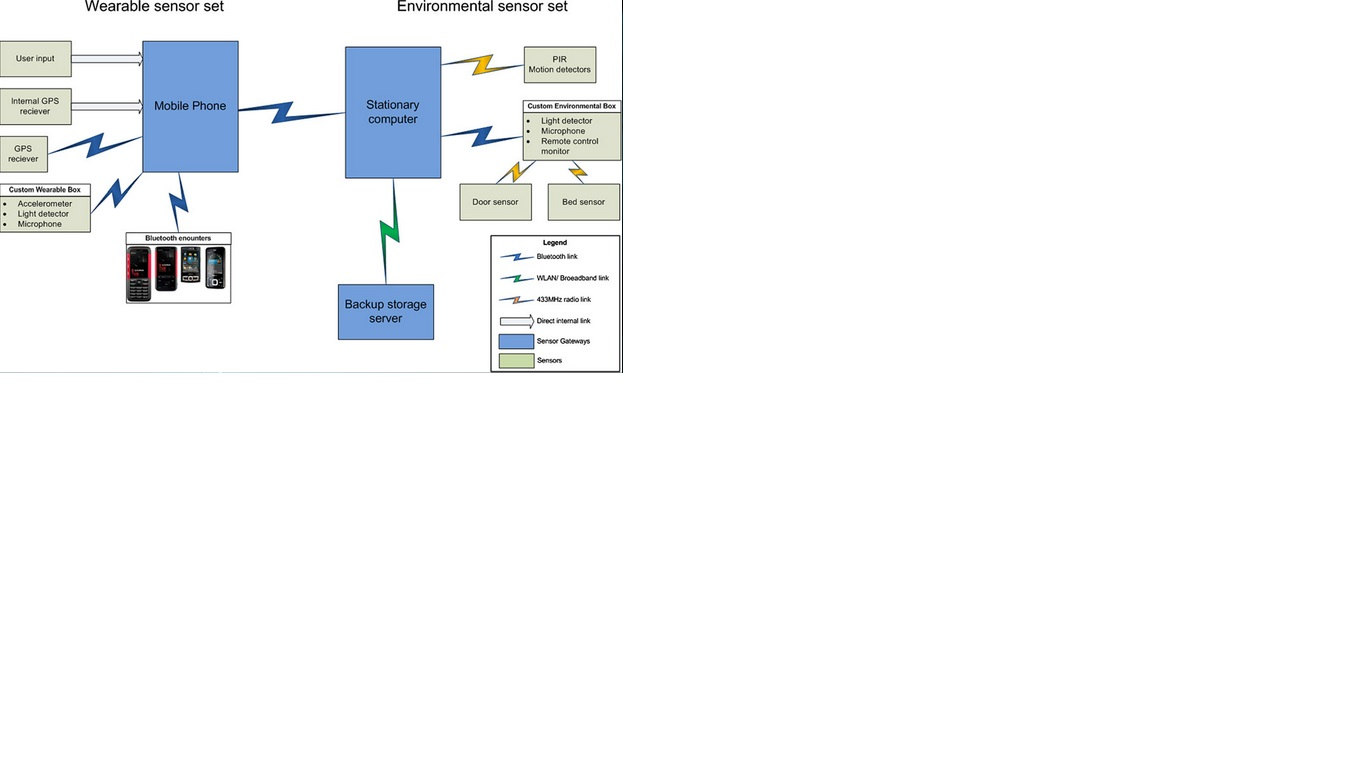
\includegraphics[width=0.5\textwidth]{images/psychic}}
  \caption{Schemat aplikacji badającej zachowania pacjenta chorego psychicznie}
\end{figure}
\section{Akcelerometr  w leczeniu choroby parkinsona}
Również choroby neurodegeneracyjne mają swoją szufladę w dziedzinie rozwoju technologii mHealth. Badania pokazują (\cite{AICPSSanders2013RemotesmartphonemonitoringformanagementofParkinsonsDiseaseEEGaccelerationactivitymonitoringelectroencephalogrammobilecomputingsensorsmart-phonewatchwrist}), iż regularne monitorowanie stanu zdrowia pacjenta może znacznie opóźnić rozwój choroby. Niestety częste wizyty w szpitalu dla wielu pacjentów są nieomal nieosiągalne. Dlatego też podręczne urządzenia, takie jak smartphone'y, okazują się tu nieocenione.